\documentclass[../writeup.tex]{subfiles}

\begin{document}  



\section{The Two-Bucket Camera}

\subsection{Notations}

The coded two-bucket (C2B) camera is a pixel-wise coded exposure camera that outputs two images in a single exposure.\cite{weiCodedTwoBucketCameras2018} Each pixel in the sensor has two photo-collecting site, i.e. the two \textit{buckets}, as well as a 1-bit writable memory controlling which bucket is actively collecting light. It was shown previously that C2B camera is capable of one-shot 3D reconstruction by solving a simpler image demosaicing and illumination demultiplexing problem instead of a difficult 3D reconstruction problem. We summarize the following notations relevant to discussion

\begin{table}[!htbp]
    \begin{center}
    \begin{tabular}{rll}
        \multicolumn{1}{r}{\bf} & \multicolumn{1}{l}{\bf Notation}   &\multicolumn{1}{l}{\bf Meaning}\\
        \hline \\
                             & F                                       & number of video frames \\
                             & P                                       & number of pixels \\
                             & S                                       & number of sub-frames \\
                             & h,w                                     & dimension of image \\
        $P\times F\times S$  & $\bC$                                   & code tensor \\
        $P\times 1\times S$  & $\widetilde{\bC}$                       & 1-frame code tensor that spatially multiplex $F$ frame tensor $\bC$ \\
        $F\times S$          & $\bC^p$                                 & activity of bucket 0 pixel $p$ cross all frames and sub-frames \\
        $F\times S$          & $\overline{\bC}^p$                       & activity of bucket 1 pixel $p$ cross all frames and sub-frames \\
        $1\times S$          & $\bc^p_f$                               & active bucket of pixel $p$ in the sub-frames of frame $f$ \\
        $1\times L$          & $\bl_s$                                 & scene's illumination condition in sub-frame $s$ of every frame \\
        $P\times S$          & $\bC_f=[\bc_1^p;\cdots;\bc_F^p]$        & activity of bucket activity of all pixels across all sub-frames of $f$ \\
        $S\times L$          & $\bL= [\bl_1;\cdots;\bl_S]$             & time-varying illumination condition (same for all frames) \\
        $2F\times S$         & $\bW$                                   & optimal bucket multiplexing matrix \\
                             & $\bt^p$                                 & transport vector at pixel $p$ \\
        $F \times 1$         & $\bi^p,\hat{\bi}^p$                     & measured two-bucket intensity at pixel $p$ in $F$ frames \\
        $F \times 1$         & $r,\hat{r}$                             & illumination ratios at pixel $p$ in $F$ frames \\
        $F\times P$          & $\bI = [\bi^1 \cdots \bi^P],\hat{\bI}$  & two-bucket image sequence in $F$ frames \\ 
        $P\times 2F$         & $\sI = [\bI^T \;\hat{\bI}^T]$           & two-bucket image sequence \\
        $P\times 2$          & $\bY$                                   & two-bucket illumination mosaic \\
        $S\times 1$          & $\si^p$                                 & pixel intensity under $S$ illuminations at pixel $p$ \\
        $P\times S$          & $\bX = [\si^1 \cdots \si^P]^T$          & pixel intensity under $S$ illuminations \\    
        $2P\times 1$         & $\by = \vec{\bY}$                       & vectorized two-bucket illumination mosaic \\
        $SP\times 1$         & $\bx = \vec{\bX}$                       & vectorized pixel intensity under $S$ illumiantions \\
        $2P\times 2PF$       & $\bB$                                   & subsampling linear map \\
        $2P\times SP$        & $\bA = \bB(\bW\otimes \bI_P)$           & illumination multiplexing and subsampling linear map \\
    \end{tabular}
    \end{center}
\end{table}
\noindent Illumination ratios are albedo \textit{quasi-invariant}, a property which can be exploited for downstream processing
\[
    r = \frac{\bi^p[f]}{\bi^p[f] + \hat{\bi}^p[f]} 
    \quad\quad
    \hat{r} =   \frac{\hat{\bi}^p[f]}{\bi^p[f] + \hat{\bi}^p[f]} 
\]

\begin{figure}[h!]
    \begin{center}
        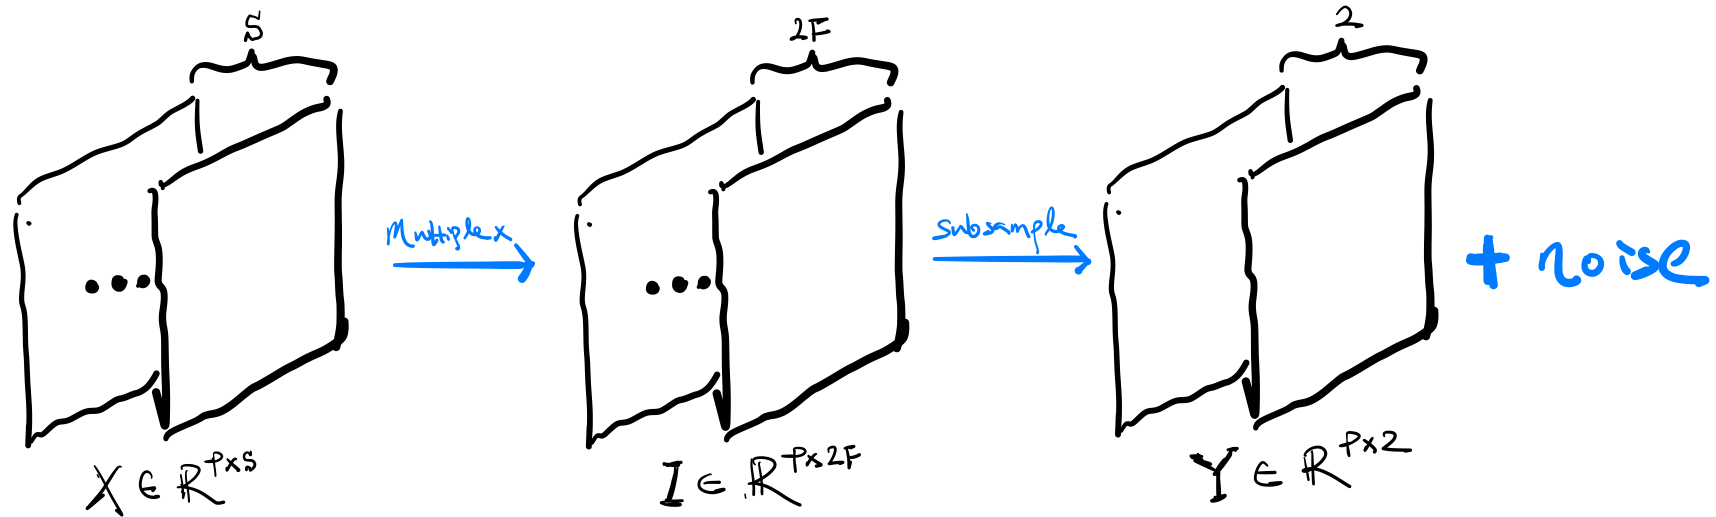
\includegraphics[width=5in]{image_formation_schema}
    \end{center}
    \caption{Image Formation Sketch}
    \label{fig:image_formation_schema}
\end{figure}

\subsection{The Forward Image Model}

\paragraph{Subsampling Mapping}
Let $\bS \in \{1,2,\cdots,F\}^P$ be a vector specifying how the one-frame code tensor $\widetilde{\bC}$ is constructed, i.e. $\tilde{\bc}_1^{p} := \bc_{\bS_p}^p$, for all pixels $p$. We can view $\bS$ as a mask to construct a \textbf{S}ubsampling linear map that maps vectorized two-bucket image sequences $\sI$ to the vectorized illumination mosaics $\bY$. In particular, let $\bB' \in \R^{P\times PF}$ and $\bB \in \R^{2P \times 2PF}$ be defined as follows 
\begin{align*}
    \bB' &=
    \begin{bmatrix}
        \diag{\mathbbm{1}_{\{1\}}(\bS) } & \diag{\mathbbm{1}_{\{2\}}(\bS) } & \cdots & \diag{\mathbbm{1}_{\{F\}}(\bS) }
    \end{bmatrix} \\
    \bB &=  \bI_2 \otimes \bB' = 
    \begin{bmatrix}
        \bB' & \mathbf{0} \\
        \mathbf{0} & \bB' \\
    \end{bmatrix}
\end{align*}
Then we have the following relation between $\sI$ and $\bY$,
\begin{equation}
    \label{eq:subsampling_relation}
    \vec{\bY} = \bB \vec{\sI}
\end{equation}
In essence, $\bB$ is a linear operator that trade spatial resolution (measures $\frac{1}{F}$ of the pixels for each frame) for temporal resolution (one two-bucket shot instead of acquiring $F$ frames). We can think of a parallel in RGB color imaging, where bayer mosaic trade spatial resolution for spectral resolution. As an example when $F=3$ and $P=4$, the corresponding $\bS$, when reshaped to dimension of a $2\times 2$ image, and single image subsampling linear map $\bB'$ are given by
\[
    \bS = 
    \begin{bmatrix}
        1 & 2 \\
        2 & 3
    \end{bmatrix}    
    \qquad
    \bB' = 
    \begin{bmatrix}
        1& 0& 0& 0& 0& 0& 0& 0& 0& 0& 0& 0 \\
        0& 0& 0& 0& 0& 1& 0& 0& 0& 0& 0& 0 \\
        0& 0& 0& 0& 0& 0& 1& 0& 0& 0& 0& 0 \\
        0& 0& 0& 0& 0& 0& 0& 0& 0& 0& 0& 1 \\
    \end{bmatrix}
\]

\paragraph{Image Formation}
Per-pixel image formation model is
\[
    \begin{bmatrix}
        \bi^p \\ \hat{\bi}^p
    \end{bmatrix}
    = 
    \begin{bmatrix}
        \bC^p \\ \overline{\bC}^p
    \end{bmatrix}
    \begin{bmatrix}
        \bl_1 \bt^p \\ \vdots \\ \bl_S \bt^p
    \end{bmatrix}
    = 
    \begin{bmatrix}
        \bC^p \\ \overline{\bC}^p
    \end{bmatrix}
    \si^p
\]
If bucket activity is same for all pixels and we use the optimal bucket multiplexing matrix $\bW$, we can write the above linear relationship compactly for all pixels as
\begin{equation}
    \label{eq:image_formation}
    \sI = \bX \bW^T
\end{equation}
As shown in Figure~\ref{fig:image_formation_schema}, illumination multiplexing and spatial subsampling can be combined to obtain a single linear function that maps images under $S$ different illuminations $\bX$ to the two-bucket images $\bY$. From (\ref{eq:subsampling_relation}) and (\ref{eq:image_formation}), there exists a linear relationship between $\bx$ and $\by$, 
\begin{equation}
    \label{eq:linear_mapping}
    \by = \bB \vec{\sI} = \bB \vec{\bX \bW^T} = \bB(\bW \otimes \bI_P) \vec{\bX} = \bA\bx
\end{equation}
where $\bA \in \R^{2P\times SP}$ be a linear map that illumination multiplexes and subsamples $\bX$,
\[
    \bA = \bB(\bW\otimes \bI_P)
\]
and $\bI_P\in\R^{P\times P}$ is identity. 

\subsection{Image Processing Pipeline}
The reconstruction pipeline is as follows
\begin{enumerate}
    \item Use $\widetilde{\bC}$ for bucket activities and capture the two-bucket image $\bY$
    \item upsample the images to full resolution images $\sI$
    \item demultiplex $\sI$ to obtain $S$ full resolution images $\bX$ as a least squares solution to a (\ref{eq:image_formation})
    \item use $\bX$ to solve for disparity and albedo
\end{enumerate}
Step 2 and 3 are critical to downstream reconstuctions. When $S=3,S=4$ and $\bS$ being analogous to bayer mask, we can upsample the images using standard demosaicing algorithms. However, it is not immediately obvious to extend demosaicing methods to support arbitrary $\bS$, or more specifically, for scenarios where the spatial subsampling scheme is not bayer and when number of frames is not 3. One approach which we consider later involves the following steps
\begin{enumerate}
    \item Use $\widetilde{\bC}$ for bucket activities and capture the two-bucket image $\bY$
    \item Recover full resolution images $\bX$ under $S$ illuminations from $\bY$ by solving a linear inverse problem
    \item use $\bX$ to solve for disparity and albedo
\end{enumerate}


\end{document}